\begin{frame}[fragile]{Soft-Margin Assumption}
  \textcolor{lightgray}{Dual form of the primary Lagrangian problem:}
  \newline
  \begin{equation*}
    \begin{split}
      \textcolor{lightgray}{\max_{\alpha}\ \sum_{i=1}^{L} \alpha_i - \frac{1}{2} \alpha^T H \alpha}
    \end{split}
  \end{equation*}

  subject to:
  \newline
  \begin{equation*}
    \textcolor{lightgray}{\sum_{i=1}^{L} \alpha_i y_i = 0 \hspace{.5cm} \text{and}}
    \hspace{.5cm} 
    \textcolor{blue}{\forall_i\ \mathbf{C \geq \alpha_i \geq 0}}
  \end{equation*}

  \vspace{.3cm}

  where $\mathbf{C}$ controls the trade-off between the slack variable penalty 
  and the size of the margin (a low $\mathbf{C}$ makes the hyperplane decision 
  surface smooth, while a high $\mathbf{C}$ aims at classifying all points correctly).
\end{frame}

\begin{frame}[fragile]{Hard-Margin vs Soft-Margin}
  \begin{columns}[onlytextwidth, T, c]
    \begin{column}{.5\textwidth}
        \begin{figure}
            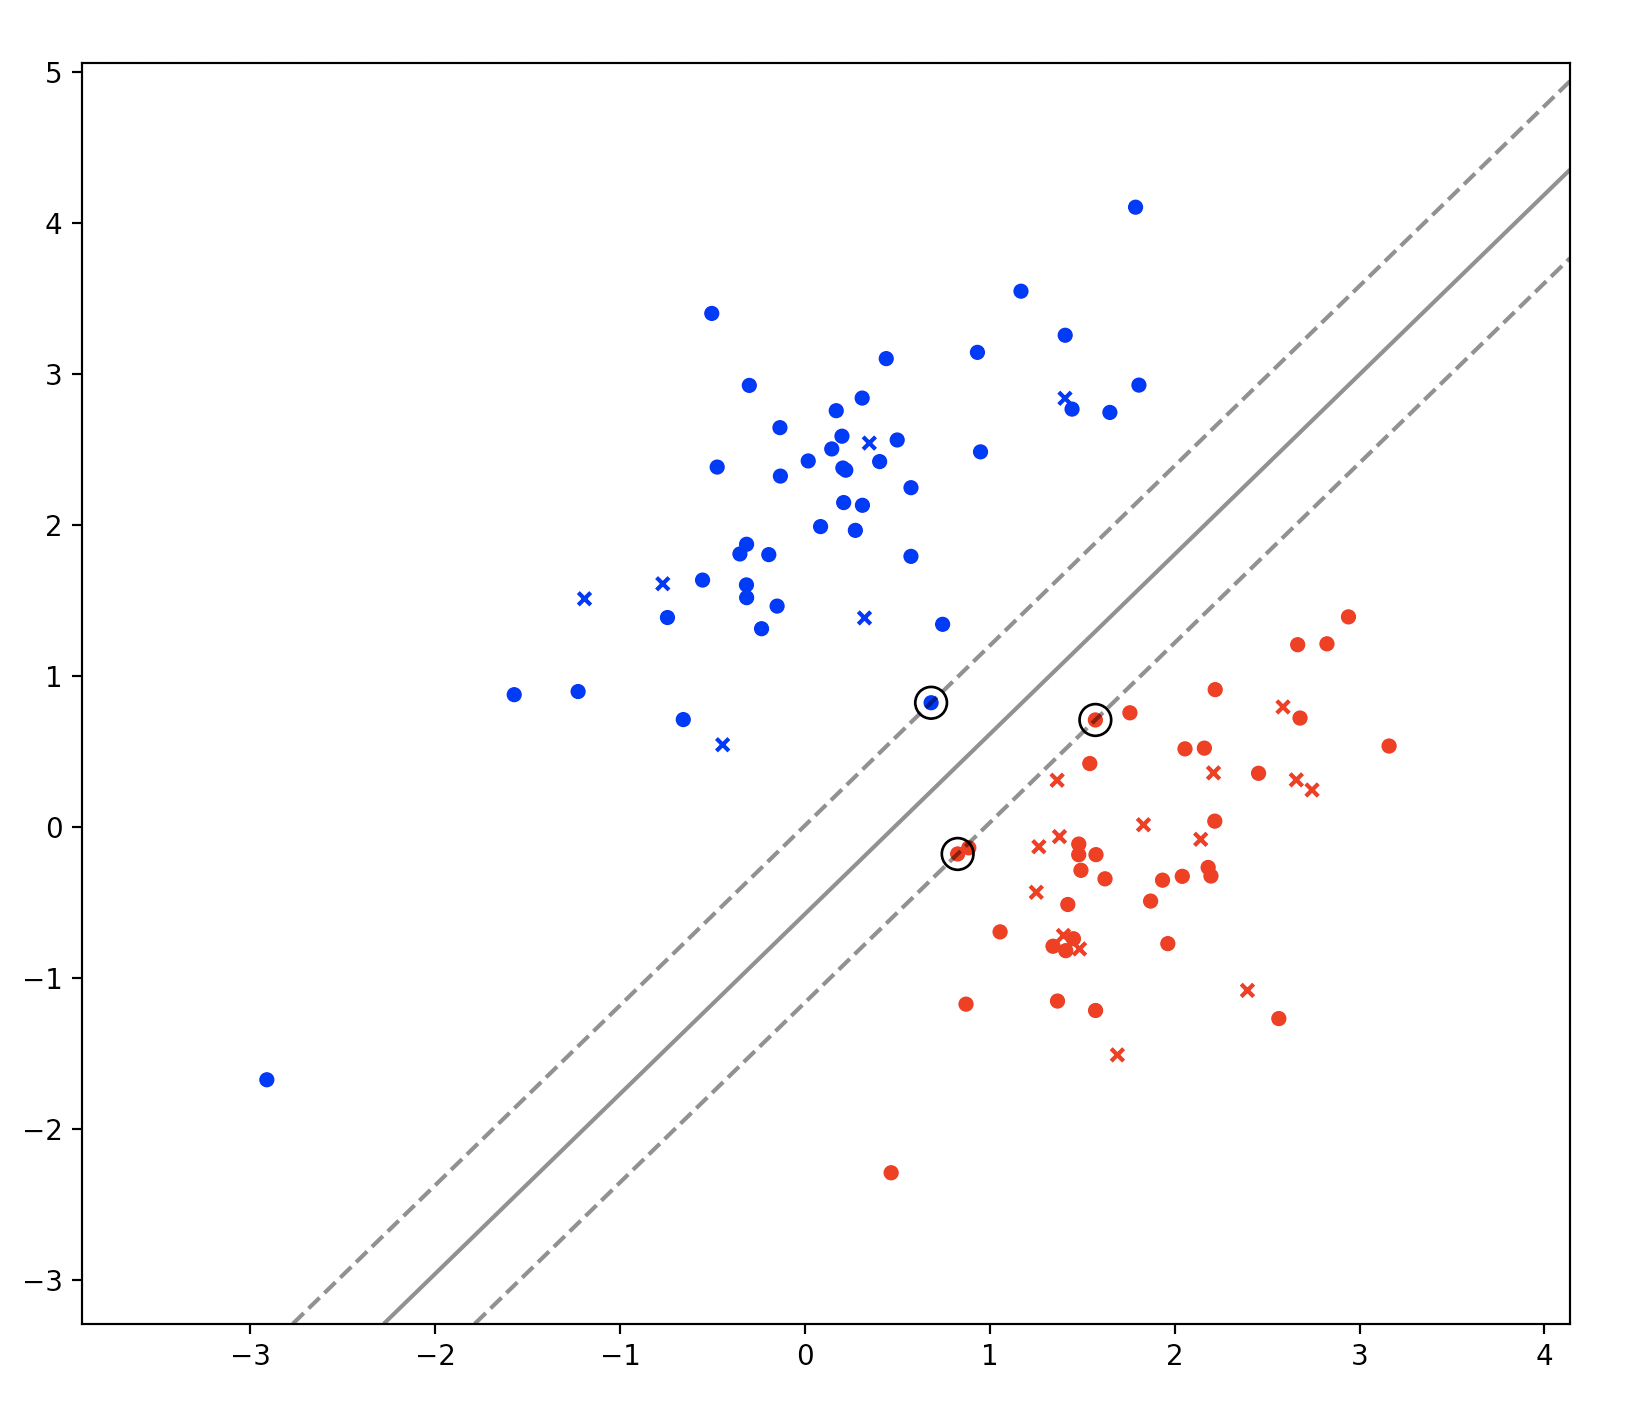
\includegraphics[width=5cm]{assets/images/s3.01.png}
            \caption{Hard-Margin}
        \end{figure}
    \end{column}
    \begin{column}{.5\textwidth}
        \begin{figure}
            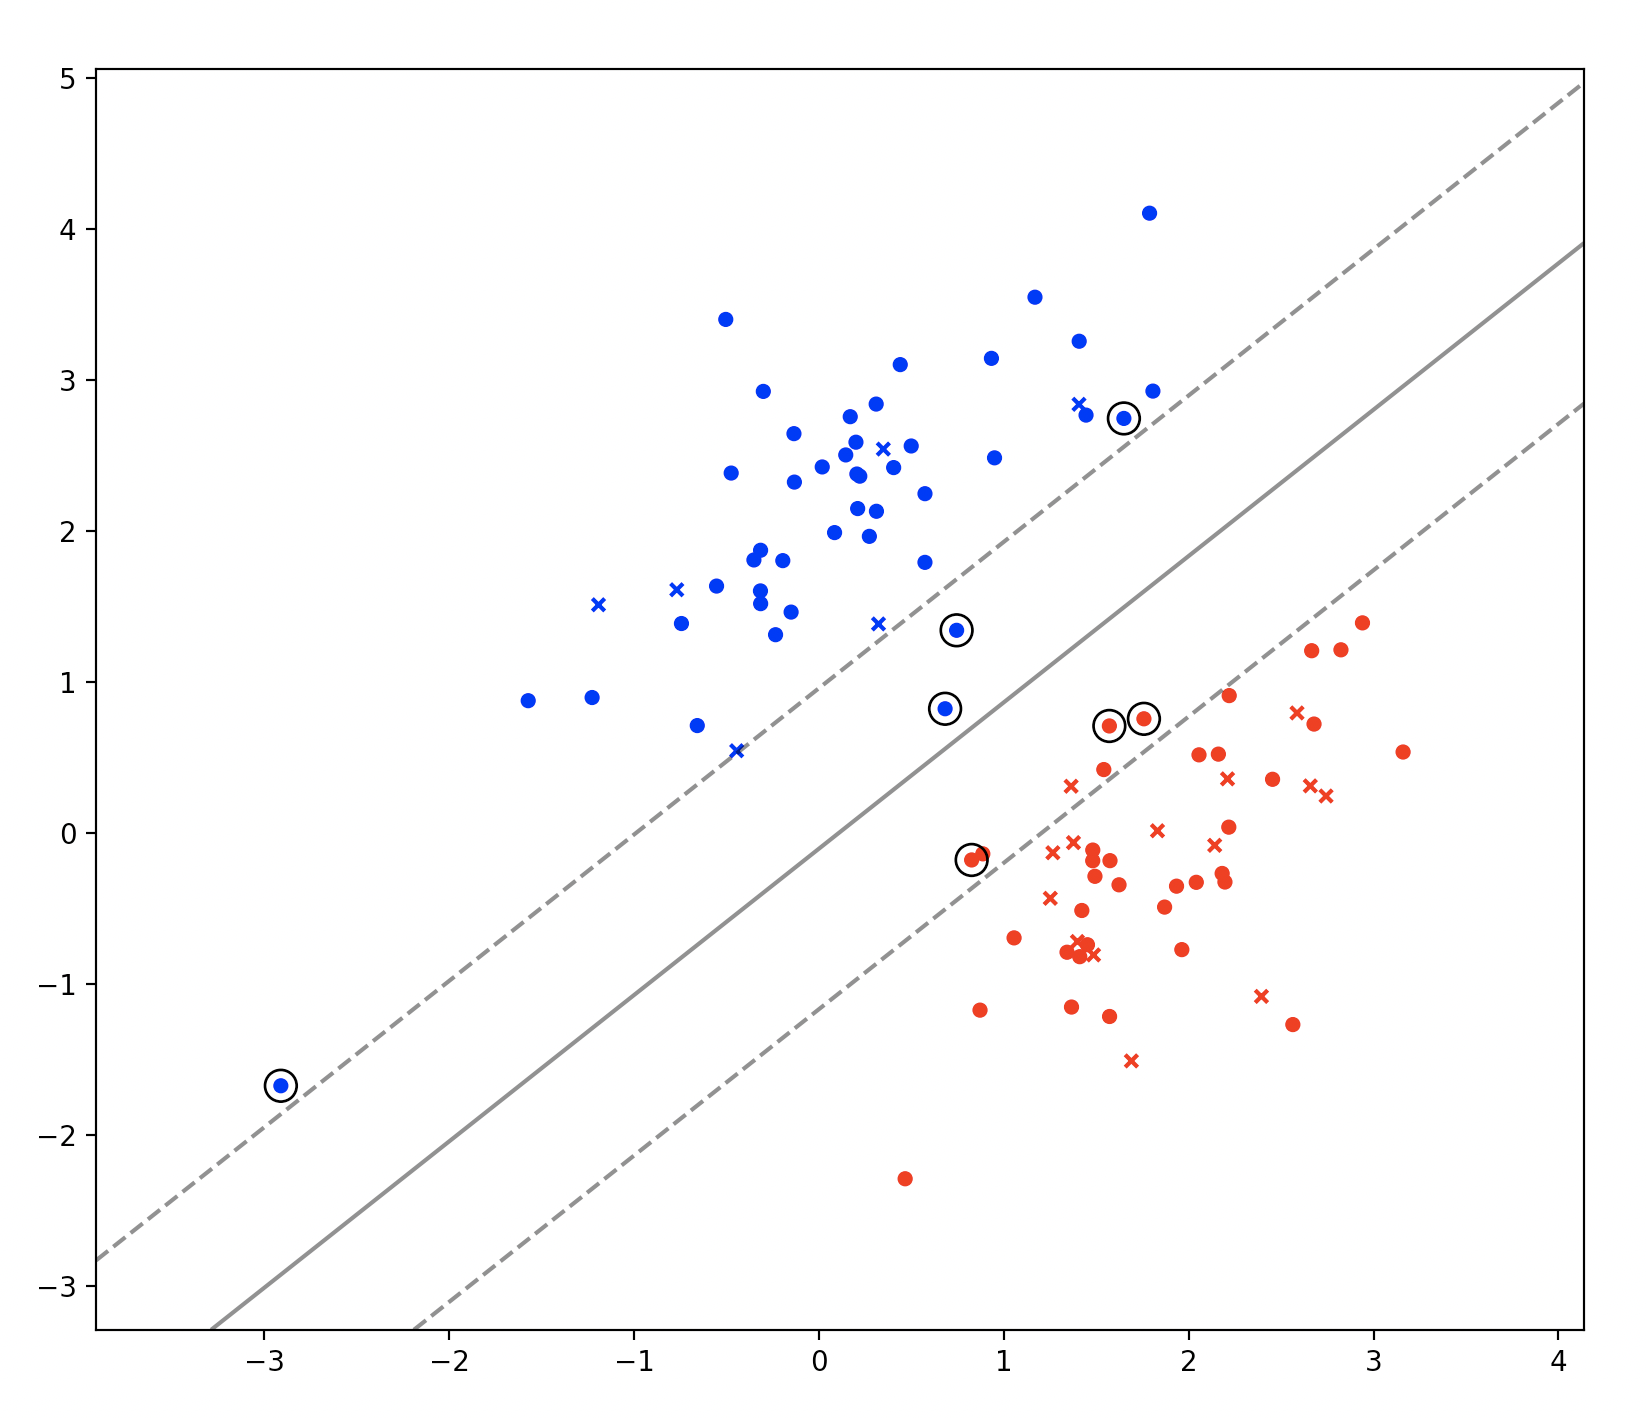
\includegraphics[width=5cm]{assets/images/s3.02.png}
            \caption{Soft-Margin}
        \end{figure}
    \end{column}    
  \end{columns}
\end{frame}
